\documentclass[../../main.tex]{subfiles}

\begin{document}
\problem{21}
\begin{wts}
What is the maximum number of bytes that can be included in a UDP payload?  (Hint: the answer to this question can be determined by your previous answer) 
\end{wts}

\begin{proof}
    Consider the following graphic,\\
    %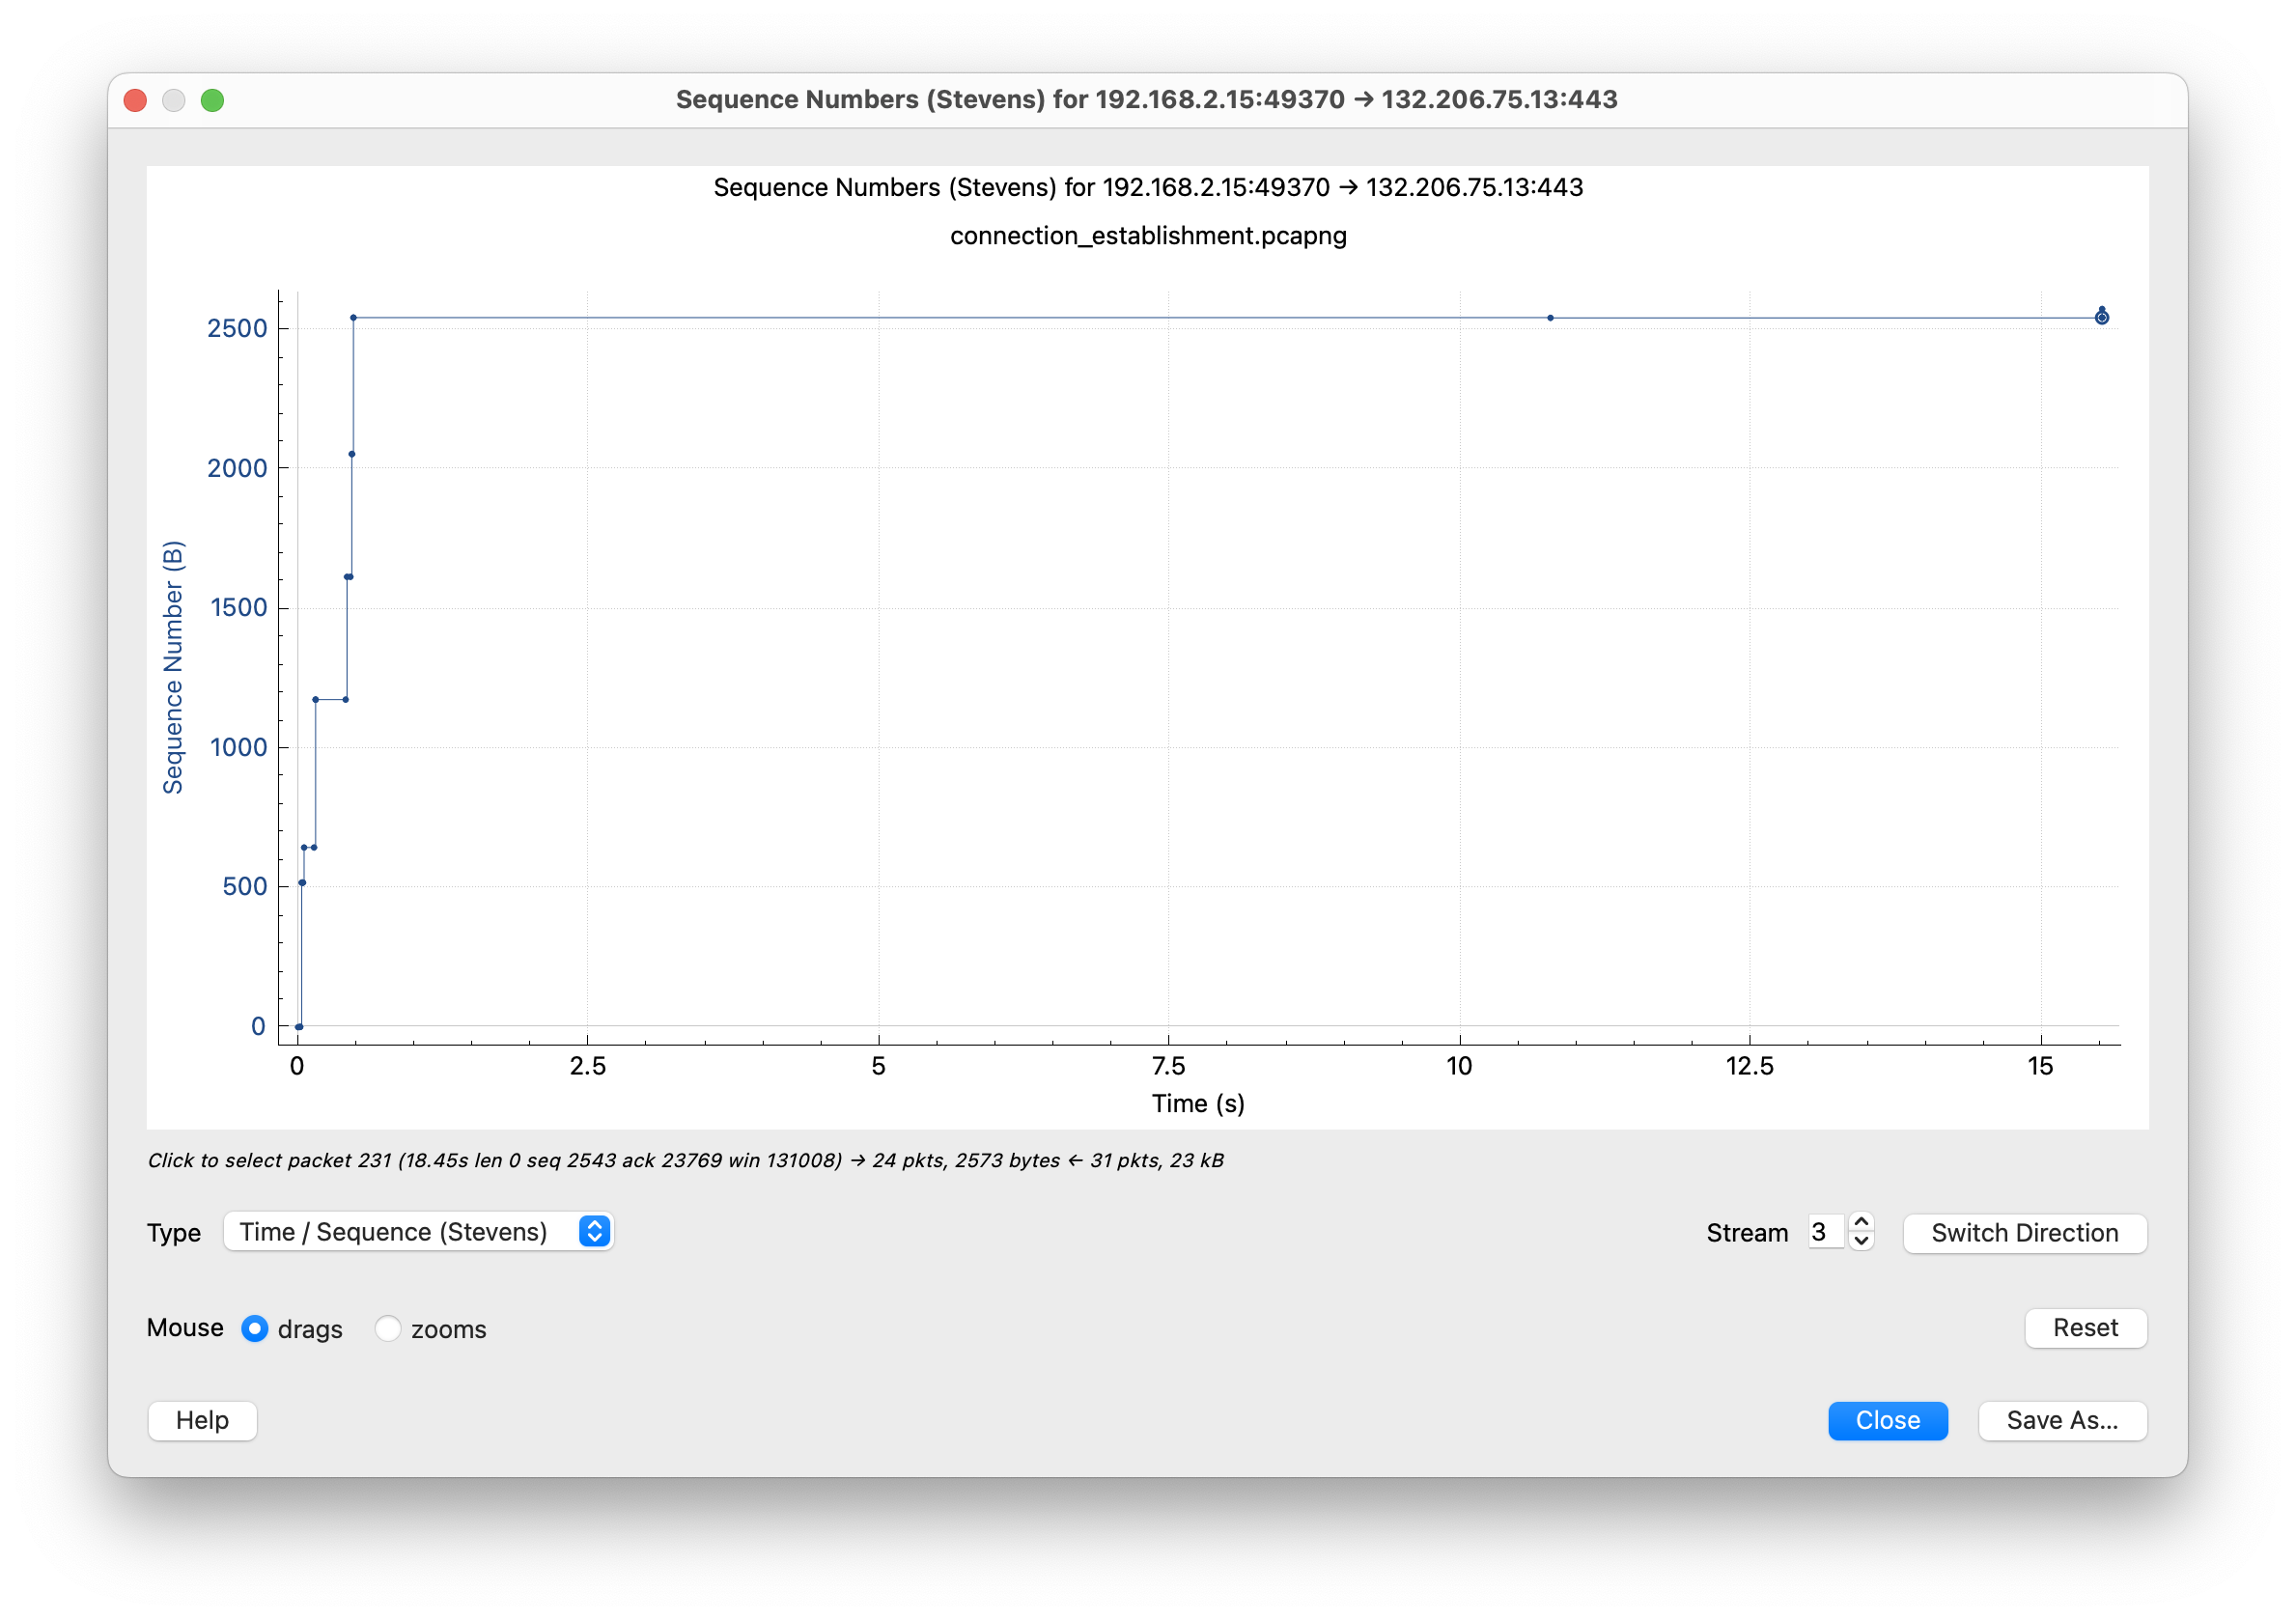
\includegraphics[width=\textwidth]{subfiles/images/connection_bytestream_plot_Q19_client_to_server.png}
    If we focus our attention towards the segments of significant lengths, then obviously the congestion avoidance phase never takes over. Since the increase in the sequence numbers do not decrease. However, this is but a pathological case in Reliable Data Transfer, as the number of bytes that are exchanged between the client and server are small. (The webpage is quite light-weight).\\
    
    Since no packets are dropped, the congestion window does not experience a significant decrease.
\end{proof}

\end{document}